%  LaTeX support: latex@mdpi.com 
%  For support, please attach all files needed for compiling as well as the log file, and specify your operating system, LaTeX version, and LaTeX editor.

%=================================================================
\documentclass[entropy,article,submit,pdftex,moreauthors]{Definitions/mdpi} 

%=================================================================
% MDPI internal commands - do not modify
\firstpage{1} 
\makeatletter 
\setcounter{page}{\@firstpage} 
\makeatother
\pubvolume{1}
\issuenum{1}
\articlenumber{0}
\pubyear{2024}
\copyrightyear{2024}
%\externaleditor{Academic Editor: Firstname Lastname}
\datereceived{ } 
\daterevised{ } % Comment out if no revised date
\dateaccepted{ } 
\datepublished{ } 
%\datecorrected{} % For corrected papers: "Corrected: XXX" date in the original paper.
%\dateretracted{} % For corrected papers: "Retracted: XXX" date in the original paper.
\hreflink{https://doi.org/} % If needed use \linebreak
%\doinum{}
%\pdfoutput=1 % Uncommented for upload to arXiv.org
%\CorrStatement{yes}  % For updates


%=================================================================
% Add packages and commands here. The following packages are loaded in our class file: fontenc, inputenc, calc, indentfirst, fancyhdr, graphicx, epstopdf, lastpage, ifthen, float, amsmath, amssymb, lineno, setspace, enumitem, mathpazo, booktabs, titlesec, etoolbox, tabto, xcolor, colortbl, soul, multirow, microtype, tikz, totcount, changepage, attrib, upgreek, array, tabularx, pbox, ragged2e, tocloft, marginnote, marginfix, enotez, amsthm, natbib, hyperref, cleveref, scrextend, url, geometry, newfloat, caption, draftwatermark, seqsplit
% cleveref: load \crefname definitions after \begin{document}

%=================================================================
% Please use the following mathematics environments: Theorem, Lemma, Corollary, Proposition, Characterization, Property, Problem, Example, ExamplesandDefinitions, Hypothesis, Remark, Definition, Notation, Assumption
%% For proofs, please use the proof environment (the amsthm package is loaded by the MDPI class).

%=================================================================
% Full title of the paper (Capitalized)
\Title{How Information Evolves}

% MDPI internal command: Title for citation in the left column
\TitleCitation{How Information Evolves}

% Authors, for the paper (add full first names)
\Author{Dan Adler $^{1}$}

%\longauthorlist{no}

% MDPI internal command: Authors, for metadata in PDF
\AuthorNames{Dan Adler}

% MDPI internal command: Authors, for citation in the left column
\AuthorCitation{Dan Adler}
% If this is a Chicago style journal: Lastname, Firstname, Firstname Lastname, and Firstname Lastname.

% Affiliations / Addresses (Add [1] after \address if there is only one affiliation.)
\address{%
$^{1}$ \quad dan@danadler.com}

%\simplesumm{} % Simple summary

%\conference{} % An extended version of a conference paper

% Abstract (Do not insert blank lines, i.e. \\) 
\abstract{Evolution is a fundamental process of life, requiring a population of replicating entities capable of adaptation, governed by fitness-driven selection. In this paper, we explore a form of abiotic evolution, demonstrating how probability imbalance, feedback loops, and population dynamics can drive the emergence of ordered patterns without reliance on specific physical laws. Through abstract, non-physical systems of symbolic tokens governed by local probabilistic interactions, we show how imbalances in frequency and stability create feedback loops that produce emergent complexity. We discuss how these mechanisms mix top-down and bottom-up causality. Our findings provide insights into the principles of pattern formation across biological, chemical, and abstract systems. This study highlights that emergent complexity is a universal property of systems with probabilistic interactions and selection mechanisms, offering a new perspective on the origins of pattern formation beyond the constraints of physical determinism.}

% Keywords
\keyword{Abiotic evolution; emergence; information theory; entropy; randomness; pattern formation; universal evolution;  stability; feedback loops; Bayesian reasoning; top-down causality; symbolic systems; complex systems}

\graphicspath{{images/}}

%%%%%%%%%%%%%%%%%%%%%%%%%%%%%%%%%%%%%%%%%%
\begin{document}
%%%%%%%%%%%%%%%%%%%%%%%%%%%%%%%%%%%%%%%%%%

% The order of the section titles is different for some journals. Please refer to the "Instructions for Authors” on the journal homepage.

\section{Introduction}

The study of evolution, complexity, and information has long been a cornerstone of multiple scientific disciplines, bridging physics, biology, and computation. Foundational works such as Schrödinger's \textit{What is Life?} \cite{schrodinger1944life} posed fundamental questions about how order emerges from disorder, inspiring theoretical explorations of how physical laws govern the emergence of biological systems. Similarly, Tegmark's \textit{Mathematical Universe Hypothesis} \cite{tegmark2008mathematical} posits that the universe itself is a mathematical structure, where physical phenomena are manifestations of abstract mathematical rules. These works frame the question of complexity but often leave the detailed mechanisms of emergence unaddressed.

In the realm of evolutionary dynamics, Nowak's seminal text \textit{Evolutionary Dynamics} \cite{nowak2006evolutionary} provides rigorous mathematical models that describe the mechanisms of replication, mutation, and selection. While these models illuminate the principles of biological evolution, they assume the existence of self-replicating entities and do not delve into how such entities might arise from purely abiotic processes. Similarly, Wheeler's concept of "It from Bit" \cite{wheeler1990itbit} intriguingly suggests that information underpins the physical world, but it lacks a concrete mechanism for how information structures form and evolve.

Dennis Noble's work on top-down causality \cite{noble2012causality} emphasizes the role of systems-level behavior in determining lower-level interactions. This perspective challenges reductionist paradigms but does not address how such systems might emerge from simpler, abiotic conditions. On the computational side, Seth Lloyd’s concept of the universe as a quantum computer \cite{lloyd2006programming} provides a framework for understanding the universe as a computational entity but leaves open the question of how specific computational rules or patterns arise.

Algorithmic complexity and Shannon’s information theory \cite{shannon1948mathematical} provide powerful tools for quantifying information and complexity but do not explain how information is created or evolves within physical systems. These frameworks focus on static measures of complexity, often missing the dynamic interplay between interactions and selection that drives the formation of ordered structures.

The approach proposed in this paper distinguishes itself by focusing on ABC systems, which offer an explicit, abstract model for the emergence of complexity and information. Unlike prior work that remains tied to specific physical systems or abstract concepts without implementation pathways, ABC systems provide a mechanism for how stable patterns arise, evolve, and persist based solely on probabilistic interactions and stability constraints. By abstracting out the specific physics of the system, ABC systems offer a universal framework applicable to a wide range of phenomena, from chemical interactions to computational models.

In contrast to Wheeler’s "It from Bit," which lacks a generative mechanism, ABC systems demonstrate how information structures emerge dynamically through selection pressures. Unlike evolutionary dynamics as formulated by Nowak, which assumes pre-existing replicators, ABC systems show how stable, self-replicating patterns can arise from purely abiotic interactions. Furthermore, the framework of ABC systems provides a path to connect the abstract ideas of Lloyd and Tegmark with practical, realizable dynamics, where probabilistic interactions evolve into ordered patterns encoding information.

This paper advances the field by demonstrating how the principles of stability-driven selection, feedback, and interaction probabilities can generate complexity and information in a way that bridges abiotic and biotic systems. By providing a detailed mechanism for the emergence of order, this work extends prior theories into a practical and computationally realizable framework.


\section{ABC System Fundamentals}

This paper considers "ABC Systems" defined as follows: a population of elements \( A, B, C, \dots \) capable of forming compounds through local interactions of unspecified forces. These elements could exist in our physical universe, or in an abstract universe. The stability of compounds determines how many generations they will persist, and we assume the base elements regenerate. Over successive generations, the system undergoes a form of natural selection where compound stability drives the evolution of the population. ABC systems are governed by two distinct but interrelated probability distributions: The population distribution, reflecting the relative abundance of patterns in the system, and the stability distribution, representing the likelihood that interactions between patterns are successful and result in new, stable patterns. Together, these distributions determine the dynamics of the system, including the selection of stable patterns, their evolution over generations, and the emergent information encoded within the system.

Consider a population of 3 elements: {A, B, C}. Assume B-compounds are more stable than those without B. Thus AB, BC, ABC, have a higher stability than AC or A or C. Therefore, B-compounds will persist over multiple generations, while the others will quickly dissipate. The more stable B-compounds will interact more frequently due to their relative frequency, even without replication or inheritance. A simulation may look like this:

\begin{figure}[htp]
    \centering
    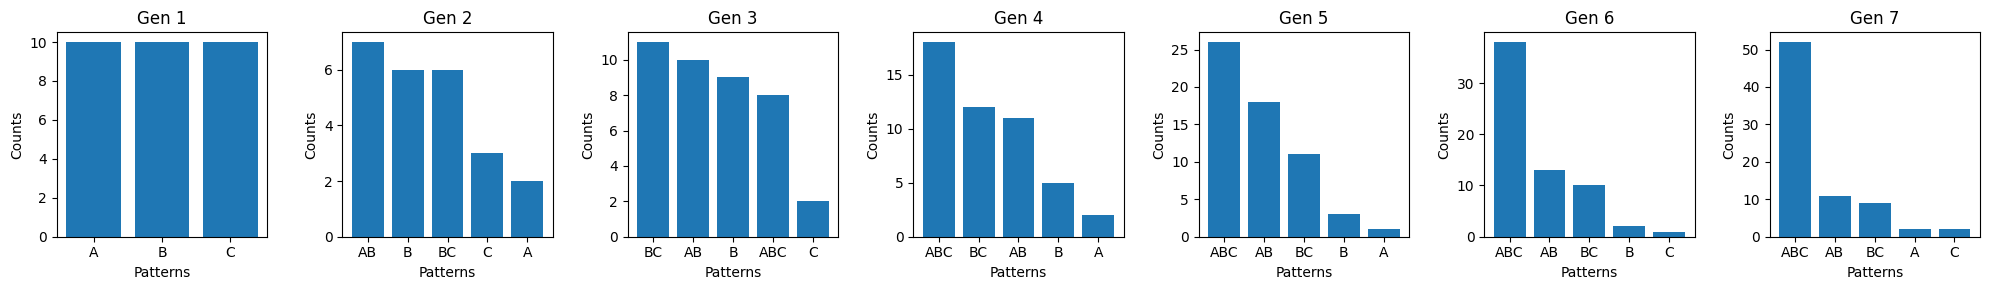
\includegraphics[width=13cm]{pat_1}
    \caption{ABC System population evolution simulation}
    \label{fig:pat_1}
\end{figure}

Where is Maxwell's demon \cite{leff2002maxwell} hiding in this example, driving it towards a low-entropy state? The answer lies in the roulette wheel. Compounds that persist longer have more chances to interact. As their frequency in the population grows, their chances to interact grow even more. In Evolutionary Dynamics, this is called fitness-proportionate selection \cite{back1996evolutionary} or roulette wheel selection \cite{goldberg1989genetic} \cite{holland1975adaptation}.

\section{Dual Probability Distributions Governing ABC Systems}

ABC systems can be effectively described by two interdependent probability distributions: the \textbf{population distribution}, which represents the relative abundance of patterns in the system, and the \textbf{stability distribution}, which quantifies the likelihood of successful interactions between patterns and the resulting stability of those interactions. These distributions interact to drive the system's dynamics, determining which patterns persist, dominate, or dissipate over time.

The population distribution reflects the probabilities of patterns at any given generation \( t \). Let \( P(p_t) \) represent the probability of pattern \( p \) in the population at time \( t \):
\[
P(p_t) = \frac{N(p_t)}{\sum_{q \in P} N(q_t)},
\]
where \( N(p_t) \) is the absolute count of pattern \( p \) in the population at time \( t \), and \( \sum_{q \in P} N(q_t) \) is the total population size at time \( t \), ensuring normalization (\( \sum_{p \in P} P(p_t) = 1 \)). The population distribution evolves over generations as patterns interact and new stable configurations emerge. As patterns with higher stability and frequent interactions become more prominent in the population, the population distribution evolves to reflects the history of past interactions and selection pressures.

The stability distribution represents the likelihood of successful interactions between patterns \( p \) and \( q \). Let \( S(p, q) \) denote the stability of the interaction between \( p \) and \( q \), defined as:
\[
S(p, q) = P(r | p, q),
\]
where \( P(r | p, q) \) is the conditional probability of forming pattern \( r \) as a result of the interaction between \( p \) and \( q \).

Stability reflects inherent properties of the patterns such as physical proximity, strength of bonds, geometric compatibility, energy barriers, or interaction rules. Stability values vary for different pairs of patterns, influencing which interactions dominate the dynamics. While the population distribution evolves rapidly, the stability distribution remains constant or changes only gradually.

\subsection{Combined Role of Population and Stability Distributions}

The two distributions together govern the dynamics of the system. The probability of two patterns \( p \) and \( q \) interacting to form a new pattern \( r \) is proportional to their population probabilities and the stability of their interaction:
\[
P(p_{t+1}) \propto P(p_t) \cdot \sum_{q \in P} P(q_t) \cdot S(p, q).
\]
The continuous-time dynamics of the feedback system can be derived as a natural extension of the discrete update equation:
\[
\frac{dP(p, t)}{dt} \approx \alpha P(p, t) \cdot S_{\text{eff}},
\]
where \( S_{\text{eff}} = \sum_{q \in P} P(q, t) \cdot S(p, q) \) is the effective stability of the pattern. Order is generated in the system through feedback-driven amplification of stable patterns. The probability of a pattern \( P(p, t) \) grows exponentially over time as a result of stabilizing interactions, following:
\[
P(p, t) \propto \exp(\alpha S_{\text{eff}} t),
\]
where \( \alpha \) is the growth rate constant, and \( S_{\text{eff}} \) is the effective stability of the pattern. This exponential growth rapidly increases the dominance of stable patterns in the population.

In contrast, random processes and stochastic fluctuations redistribute probabilities in the system, contributing to an increase in entropy. The degradation of order due to these random effects is characterized by a slower logarithmic growth in entropy:
\[
\Delta H \propto \ln(t).
\]
As time progresses, the competition between the exponential growth of stable patterns and the logarithmic increase in entropy becomes evident. The net result is that the exponential growth of order, driven by stabilizing feedback and represented as \( \exp(\alpha S_{\text{eff}} t) \), outpaces the entropy increase \( \ln(t) \). This ensures that stability-driven feedback creates a net reduction in entropy, leading the system toward a more ordered, low-entropy state. Over time, the dominance of stable patterns suppresses randomness, driving the system into configurations characterized by emergent complexity and order.

This analysis demonstrates how stability-driven interactions in local populations generate order faster than the second law of thermodynamics can degrade it. While random fluctuations tend to increase entropy, the exponential reinforcement of stable patterns creates a net reduction in entropy, leading to emergent order. The dynamics also highlight the competitive nature of the system: only patterns with sufficiently high stability and effective interaction networks survive over the long term, ensuring the self-organization of the population into ordered configurations.

\subsection{Catalysis}

Consider an ABC system where \( A \) interacts with \( B \) to form a compound \( AB \), but this interaction occurs only in the presence of a catalyst \( C \). The catalyst \( C \) is not consumed or altered during the interaction, yet it influences the system's dynamics by facilitating specific reactions. This creates selection pressure for \( C \) to persist due to its role in enabling the formation of stable compounds. In this case, the catalyst \( C \) facilitates the reaction by increasing its likelihood:
\[
P(A + B \to AB \mid C) \propto p_A \cdot p_B \cdot p_C.
\]

The catalyst \( C \) benefits indirectly, as its presence enables reactions that increase the overall fitness of the system.

\section{Interpreting Interactions as Logic Gates in ABC Systems}

ABC systems can be interpreted as encoding logical operations through their interactions, with patterns and their combinations acting as inputs and outputs of logical gates. Catalysis, a common feature in chemical systems, further reinforces this interpretation, as catalysts act as conditional enablers for specific reactions. This section explores how interactions in ABC systems can be mapped to logical operations and how catalytic behaviors correspond to logical gates or conditional statements.

\subsection{Interactions as Logical Operations}

In an ABC system, the combination of patterns can represent logical relationships. For instance, the interaction \( A + B \to AB \) can be interpreted as a logical AND operation, where \( AB \) is produced only if both \( A \) and \( B \) are present. The probabilities of patterns encode their logical "truth values," with higher probabilities corresponding to "true" states and lower probabilities corresponding to "false" states. We already showed that interaction \( A + B \to AB \) can be expressed as:
\[
P(AB) = P(A) \cdot P(B) \cdot S(AB),
\]
where \( S(AB) \) is the Stability. This is analogous to the AND operation in logic, where the output is true only if both inputs are true. Similarly, the OR operation can be represented as the dominance of either \( A \) or \( B \), given by:
\[
P(A \lor B) = P(A) + P(B) - P(A) \cdot P(B).
\]
The logical NOT operation corresponds to the absence of a pattern, represented as:
\[
P(\neg A) = 1 - P(A).
\]
These interactions collectively encode basic logical operations, enabling the system to process and store information in a manner analogous to digital logic.

\subsection{Catalysis as Conditional Logic}

In the context of ABC systems, a catalyst \( C \) facilitating the reaction \( A + B \to AB \) can be interpreted as a conditional statement or a logical gate. The presence of \( C \) determines whether the reaction occurs, making it analogous to the logical "if" condition: "If \( C \), then \( A + B \to AB \)."
This behavior maps directly to the conditional logic often found in programming and computation. In terms of probability, the catalyzed interaction can be expressed as:
\[
P(AB | C) \propto P(A) \cdot P(B) \cdot S(A, B | C),
\]
where \( S(A, B | C) \) represents the stability of the interaction in the presence of the catalyst \( C \).

Catalysts can also be compared to the gate of a transistor in an electronic circuit. Just as a transistor gate controls the flow of current between its source and drain, a catalyst \( C \) controls the occurrence of the reaction \( A + B \to AB \). The analogy extends to the amplification effect: a small amount of \( C \) can enable significant interaction between \( A \) and \( B \), similar to how a small gate voltage modulates a larger current.

Additionally, catalysts can encode more complex logical gates. For example, a two-step catalysis process \( C_1 \) and \( C_2 \) enabling \( A + B \to AB \) and \( AB + C \to ABC \) respectively corresponds to a sequential logic operation:
\[
\text{IF } C_1, \text{ THEN } A + B \to AB, \quad \text{AND IF } C_2, \text{ THEN } AB + C \to ABC.
\]
Such catalytic networks can encode conditional logic akin to nested IF statements in programming or complex gates in digital logic circuits. 

Interactions in ABC systems can be interpreted as logical operations, with catalysts playing the role of conditional gates or enabling mechanisms. This mapping reveals a computational aspect of such systems, where reactions and stability constraints naturally encode logic. Catalytic behaviors extend this logic by introducing conditionality, enabling ABC systems to perform more complex computations. These insights bridge the gap between chemical interactions and digital computation, highlighting the potential for emergent logic and information processing in abiotic systems.

\section{Generating Cellular Automata Rules in ABC Systems}

ABC systems, with their interaction-driven dynamics and stability-based selection, can be extended to generate behavior analogous to cellular automata (CA). By carefully defining interaction rules and stability imbalances, ABC systems can mimic specific CA rules, including those capable of producing complex behavior. This section demonstrates how stability imbalances in an ABC system can emulate one of Wolfram’s elementary cellular automata rules and explores the mechanisms by which these systems transition into computational models.

\subsection{Mapping ABC Systems to Cellular Automata}

Cellular automata operate on discrete states, where the next state of a cell depends on its current state and the states of its neighbors. Similarly, ABC systems evolve based on the interactions and stabilities of patterns in the population. By associating patterns in the ABC system with the states of a CA, and interactions with transition rules, we can map ABC dynamics to CA behavior.

\subsection{Stability Imbalances as Transition Rules}

In ABC systems, the stability of interactions \( S(p, q) \) determines the likelihood of forming new patterns. To emulate a specific CA rule, we assign stability imbalances that prioritize the creation of patterns corresponding to the rule’s outputs. For instance, if the CA rule specifies that a cell becomes "active" when one or both neighbors are active, we increase the stability of interactions that encode this outcome.

Let us consider an example with patterns \( A, B, C \), where \( A, B, C \) correspond to states in a 1D CA. We define stability imbalances such that:
\[
S(A, B) = 0.8, \quad S(A, C) = 0.2, \quad S(B, C) = 0.5,
\]
and these interactions map to the CA rule for determining the next state of a cell based on its neighbors.

\subsection{Example: Wolfram’s Rule 30}

Wolfram’s Rule 30 is a well-known elementary CA rule producing complex behavior. The rule specifies the following transition table:
\[
\begin{array}{ccc|c}
\text{Left} & \text{Center} & \text{Right} & \text{Next State} \\
1 & 1 & 1 & 0 \\
1 & 1 & 0 & 0 \\
1 & 0 & 1 & 0 \\
1 & 0 & 0 & 1 \\
0 & 1 & 1 & 1 \\
0 & 1 & 0 & 1 \\
0 & 0 & 1 & 1 \\
0 & 0 & 0 & 0 \\
\end{array}
\]
This can be encoded in an ABC system by associating the states of cells with patterns and defining stability imbalances to favor interactions that generate the correct next state. For example:
\begin{itemize}
    \item Define \( A, B, C \) as the current states of left, center, and right cells, respectively.
    \item Use stability imbalances to prioritize outcomes matching the rule. For instance:
    \[
    S(A, B) = 0.9 \text{ if } A = 1, B = 1; \quad S(B, C) = 0.7 \text{ if } B = 1, C = 0.
    \]
\end{itemize}

\subsection{Simulation of Rule 30 in an ABC System}

To simulate Rule 30, we initialize the ABC system with patterns corresponding to the initial state of the CA and allow it to evolve according to the stability-driven dynamics. For example:
\begin{enumerate}
    \item Initialize the system with a random distribution of \( A, B, C \) (e.g., \( 101100110 \)).
    \item Define interaction rules such as \( A + B \to AB \), with stability imbalances reflecting Rule 30’s transition table.
    \item Allow the system to iterate, updating patterns based on the outcomes of interactions.
\end{enumerate}

At each iteration, the patterns \( AB, BC, \) etc., encode the next generation of the CA. The emergent dynamics will reflect the behavior of Rule 30, with complex patterns arising over successive generations.

\subsection{Implications for Emergent Complexity}

This mapping demonstrates that ABC systems can encode and simulate cellular automata, bridging the gap between chemical-like systems and computational models. Stability imbalances provide a natural mechanism for implementing transition rules, while interaction-driven evolution ensures the system retains flexibility and adaptability. The ability of ABC systems to replicate CA behavior highlights their potential for emergent computation and complex pattern formation.

\section{Bayesian Updating in ABC Systems}

ABC systems highlight a key distinction between Bayesian updating and frequentist probabilities, illustrating their respective roles in evolving versus static systems. Bayesian updating provides a dynamic framework for incorporating new information over time, making it a hallmark of systems capable of evolution and self-organization. Frequentist probabilities, on the other hand, describe point-in-time static distributions, lacking the temporal adaptability intrinsic to evolutionary dynamics.

In ABC systems, the probability of a pattern \( p \) at generation \( t+1 \) depends on its prior probability \( P(p_t) \), the probabilities of other patterns \( P(q_t) \), and the stability of their interactions \( S(p, q) \). The update rule can be expressed as:
\[
P(p_{t+1}) = \frac{P(p_t) \cdot \sum_{q \in P} P(q_t) \cdot S(p, q)}{\sum_{p' \in P} P(p'_t) \cdot \sum_{q \in P} P(q_t) \cdot S(p', q)},
\]
where the numerator reflects the likelihood of \( p \) persisting or forming through interactions, and the denominator ensures normalization of probabilities. This is analogous to the Bayesian formula:
\[
P(H|E) = \frac{P(E|H) \cdot P(H)}{P(E)},
\]
where:
\begin{itemize}
    \item \( H \): Hypothesis (\( p \) as a pattern in the system).
    \item \( E \): Evidence (interactions \( q \) and their stabilities \( S(p, q) \)).
    \item \( P(H) \): Prior probability (\( P(p_t) \)).
    \item \( P(E|H) \): Likelihood (\( \sum_{q \in P} P(q_t) \cdot S(p, q) \)).
    \item \( P(H|E) \): Posterior probability (\( P(p_{t+1}) \)).
\end{itemize}

This iterative Bayesian updating process allows ABC systems to adapt and encode new information dynamically. The system continuously adjusts pattern probabilities to reflect the effects of interactions and stability constraints, resulting in emergent complexity and self-organization.

\section{Emergent Information vs. Pre-Designed Information in ABC Systems}

ABC systems provide a natural framework for exploring the distinction between emergent and pre-designed information. The ability of these systems to evolve patterns and mimic computational processes, such as logic gates and cellular automata (CA), highlights the role of feedback, stability imbalances, and selection pressure in generating information. This stands in contrast to systems where information is externally imposed, such as 3D-printed patterns.

\subsection{Emergent Information in ABC Systems}

Emergent information arises naturally from the interactions and feedback loops within a system. In ABC systems:
\begin{itemize}
    \item \textbf{Patterns evolve dynamically}: Stable patterns persist and dominate over time through iterative interactions, encoding the history of the system.
    \item \textbf{Selection pressure guides evolution}: Stability imbalances and probabilistic feedback ensure that only certain configurations persist, driving the system toward lower-entropy, information-rich states.
    \item \textbf{No predefined outcomes}: The system explores a vast configuration space, with the resulting patterns depending on initial conditions, interaction rules, and stability constraints.
\end{itemize}
For example, an ABC system can evolve to mimic CA rules, such as Wolfram’s Rule 30, through stability imbalances. These patterns encode logical rules that emerge purely from system dynamics, without external input specifying the desired outcome.

\subsection{Pre-Designed Information in 3D-Printed Systems}

In contrast, pre-designed systems, such as 3D-printed compounds or pre-programmed circuits, rely on external inputs to define their structure and function:
\begin{itemize}
    \item \textbf{Information is imposed externally}: Patterns are directly specified by a designer or blueprint, with no reliance on system dynamics for their creation.
    \item \textbf{No evolutionary process}: The system does not explore configuration space; instead, it is constructed to achieve a predefined state.
    \item \textbf{Fixed outcomes}: The resulting patterns are static, with no capacity for adaptation or self-organization.
\end{itemize}
For instance, a 3D-printed version of Rule 30 would replicate the CA’s behavior exactly as designed, without any intermediate steps or emergent dynamics.

\subsection{A Hypothesis for Defining Pre-Designed Systems}

The contrast between emergent and pre-designed systems suggests a potential criterion for determining whether a system is pre-designed: the presence or absence of an evolutionary process. A system could be defined as pre-designed if:
\begin{itemize}
    \item Its configuration is entirely specified by external inputs.
    \item It lacks path dependency, with no evidence of intermediate states or evolutionary history.
    \item Its entropy dynamics are static or pre-determined, rather than dynamically evolving.
\end{itemize}

\subsection{Speculation: Toward a Framework for Detecting Pre-Designed Systems}

The ability of ABC systems to evolve patterns and encode information through feedback and stability imbalances highlights the possibility of distinguishing emergent and pre-designed systems based on their evolutionary behavior. This may provide a path toward defining whether a system is pre-designed. If a system displays emergent properties such as dynamic adaptation, path dependency, and entropy reduction, it likely evolves internally. Conversely, systems that lack these properties and achieve order without intermediate steps or feedback are more likely to be pre-designed.

This distinction could have profound implications for understanding natural systems, artificial constructs, and the origins of complex information in physical and computational systems. For instance, it may offer insights into distinguishing abiotic evolution from engineered systems, or identifying the hallmark features of life-like behavior in prebiotic chemistry.

Deep learning systems lie on a continuum between pre-designed systems and fully emergent ones:
\begin{itemize}
    \item \textbf{Pre-Designed Systems}: 3D-printed systems or fixed-rule systems, where the outcomes are entirely determined by external inputs.
    \item \textbf{Guided Evolution}: Deep learning systems, where evolution-like processes occur under strong external guidance and predefined constraints.
    \item \textbf{Emergent Evolution}: ABC systems, where patterns evolve through internal dynamics, with no externally imposed outcomes.
\end{itemize}

\section{Mixing Two ABC Systems: Information Flow and Entropy Dynamics}

Mixing two independently evolved ABC systems introduces a new dimension to their dynamics, where patterns and interactions from each system influence the other. This interaction results in the exchange of information, changes in entropy, and the potential emergence of novel patterns. By analyzing information flow and entropy in such mixed systems, we can gain deeper insights into the dynamics of evolving systems and their capacity for self-organization.

\subsection{Setup for Mixing Two ABC Systems}

Let two independently evolved ABC systems \( P_1 \) and \( P_2 \) represent populations of patterns \( \{A, B, C, \dots\} \) and \( \{X, Y, Z, \dots\} \), respectively. Each system evolves independently based on its population distribution \( P(p_t) \) and stability constraints \( S(p, q) \) for patterns \( p, q \) within the same system.

When the two systems are mixed, the patterns from \( P_1 \) and \( P_2 \) interact, allowing the formation of cross-system compounds (e.g., \( ABX, XYZ \)). Stability constraints extend to cross-system interactions, introducing new terms \( S(p, q) \) where \( p \in P_1 \) and \( q \in P_2 \). The joint system evolves based on updated probabilities reflecting both within-system and cross-system interactions.

\subsection{Entropy Dynamics in Mixed Systems}

After mixing, the joint entropy \( H_{\text{mix}}(t) \) becomes:
\[
H_{\text{mix}}(t) = -\sum_{p \in P_1 \cup P_2} P(p_t) \ln P(p_t),
\]
where \( P(p_t) \) now includes probabilities of cross-system patterns.

\paragraph{Case 1: Systems with Low Entropy Before Mixing}
If both \( P_1 \) and \( P_2 \) are in low-entropy states, characterized by dominance of stable patterns, the mixed system is likely to retain a low entropy. The interaction of well-organized patterns results in selective formation of cross-system compounds, reinforcing order.

\paragraph{Case 2: Systems with High Entropy Before Mixing}
If either \( P_1 \) or \( P_2 \) has high entropy, the mixing introduces randomness into the more ordered system. Cross-system interactions may lead to transient increases in entropy, but selection pressures favoring stable compounds can gradually reduce entropy in subsequent generations.

\paragraph{Case 3: Systems with Complementary Patterns}
When \( P_1 \) and \( P_2 \) have complementary patterns (e.g., \( P_1 \) lacks certain patterns that \( P_2 \) provides), mixing can generate new stable configurations that reduce entropy more effectively than in isolated systems. For instance, if \( P_1 = \{A, B\} \) and \( P_2 = \{X, Y\} \), the formation of \( ABX, BY, AX \) introduces novel low-entropy configurations.

\subsection{Emergent Behavior in Mixed Systems}

Mixing two ABC systems facilitates information flow and alters entropy dynamics, providing a powerful framework for studying interaction-driven complexity. The interplay between low-entropy patterns and cross-system interactions highlights the capacity of mixed systems to generate emergent order. By analyzing information flow and entropy changes, we gain insights into the mechanisms driving the evolution of coupled systems and the emergence of novel configurations. The mixing of two systems creates opportunities for emergent behavior:
\begin{itemize}
    \item \textbf{Novel Compounds}: Cross-system interactions lead to the formation of patterns like \( ABX \) that do not exist in either system independently.
    \item \textbf{Crossover Effects}: Patterns from one system stabilize or destabilize patterns in the other, modifying evolutionary trajectories.
    \item \textbf{Symbiosis}: Feedback loops between patterns in \( P_1 \) and \( P_2 \) can reinforce mutual stability, leading to new equilibrium states.
\end{itemize}

\section{The Path from Abiotic to Biotic Evolution in ABC Systems}

ABC systems provide a framework for understanding how evolutionary processes can emerge in purely abiotic contexts, offering insights into the transition from abiotic to biotic evolution. By encoding memory, leveraging feedback-driven adaptation, and fostering self-organization, these systems illustrate that evolution is not confined to living systems. Instead, it arises from fundamental principles of stability and selection, bridging the gap between non-living matter and life-like behavior.

In ABC systems, abiotic evolution is driven by stability imbalances, interaction probabilities, and selection pressures. Stable patterns persist and dominate the population over successive generations, encoding information about the system’s evolutionary history. These emergent patterns act as a form of "memory," comparable to biological inheritance but without replication or genetic material. This iterative process of pattern formation and dominance mirrors natural selection, where stability functions as the fitness criterion.

The transition from stability to self-replication represents a pivotal step toward biotic evolution. In ABC systems, stable patterns that catalyze their own formation lay the foundation for rudimentary replication. For example, a pattern such as \( AB \) might interact with other patterns to form identical copies (\( AB + A + B \to AB + AB \)), exhibiting primitive self-replication. Although this process lacks the fidelity and precision of genetic inheritance, it establishes the basis for replication. Feedback loops further enhance this process by reinforcing the stability and prevalence of self-replicating patterns. Over time, these patterns form networks of interactions, where mutual stabilization drives the emergence of increasingly complex and self-sustaining structures.

As stable patterns persist over generations, they encode information about the system's interactions and evolutionary history. This information storage, coupled with feedback-driven adaptation, allows the system to act as a rudimentary computational model. For instance, the ability of ABC systems to mimic logic gates and cellular automata demonstrates their capacity to encode and process information dynamically. The transition to biotic evolution occurs when these information-processing capabilities become more robust, enabling the system to store and utilize rules for its own replication and adaptation. This aligns with the principles of Turing machines, where patterns serve simultaneously as memory and computational units.

Biotic systems are characterized by inheritance, metabolism, and evolution. In ABC systems, inheritance is mirrored by the persistence of stable patterns over generations, which encode information about interactions and enable the transmission of system states. Metabolism is analogously represented by interactions between patterns that mimic energy flow, with stability serving as a proxy for energy efficiency. Evolution is driven by selection pressures that favor patterns enhancing system stability, leading to the gradual emergence of complexity. The critical distinction between abiotic and biotic systems lies in the emergence of self-replicating patterns with the capacity to evolve independently. When patterns begin to store and utilize information for their replication and stabilization, they transition from purely abiotic dynamics to life-like behavior.

The insights provided by ABC systems have significant implications for understanding the origins of life. These systems demonstrate how evolutionary processes can arise without predefined biological structures. The ability of ABC systems to evolve information storage, logic, and self-replication suggests a plausible pathway by which abiotic systems could transition to biotic evolution. The emergence of stable, self-replicating patterns capable of encoding memory marks a fundamental step, followed by the development of feedback loops that reinforce stability and adaptability, and the integration of information processing into increasingly complex networks. Together, these steps provide a framework for exploring how life might arise from non-living matter.

ABC systems illustrate that the principles underlying evolution are not exclusive to living organisms. Stability-driven selection, information storage, and feedback mechanisms provide a pathway for abiotic systems to transition toward biotic behavior. This framework bridges the divide between non-living matter and life, offering theoretical insights into the origins of complexity and the emergence of life-like properties in abiotic systems.


%%%%%%%%%%%%%%%%%%%%%%%%%%%%%%%%%%%%%%%%%%
\section{Materials and Methods}

Materials and Methods should be described with sufficient details to allow others to replicate and build on published results. Please note that publication of your manuscript implicates that you must make all materials, data, computer code, and protocols associated with the publication available to readers. Please disclose at the submission stage any restrictions on the availability of materials or information. New methods and protocols should be described in detail while well-established methods can be briefly described and appropriately cited.

Research manuscripts reporting large datasets that are deposited in a publicly avail-able database should specify where the data have been deposited and provide the relevant accession numbers. If the accession numbers have not yet been obtained at the time of submission, please state that they will be provided during review. They must be provided prior to publication.

Interventionary studies involving animals or humans, and other studies require ethical approval must list the authority that provided approval and the corresponding ethical approval code.
\begin{quote}
This is an example of a quote.
\end{quote}

%%%%%%%%%%%%%%%%%%%%%%%%%%%%%%%%%%%%%%%%%%
\section{Results}

This section may be divided by subheadings. It should provide a concise and precise description of the experimental results, their interpretation as well as the experimental conclusions that can be drawn.
\subsection{Subsection}
\subsubsection{Subsubsection}

Bulleted lists look like this:
\begin{itemize}
\item	First bullet;
\item	Second bullet;
\item	Third bullet.
\end{itemize}

Numbered lists can be added as follows:
\begin{enumerate}
\item	First item; 
\item	Second item;
\item	Third item.
\end{enumerate}

The text continues here. 

\subsection{Figures, Tables and Schemes}

All figures and tables should be cited in the main text as Figure~\ref{fig1}, Table~\ref{tab1}, etc.

\begin{figure}[H]

\includegraphics[width=10.5 cm]{Definitions/logo-mdpi}
\caption{This is a figure. Schemes follow the same formatting. If there are multiple panels, they should be listed as: (\textbf{a}) Description of what is contained in the first panel. (\textbf{b}) Description of what is contained in the second panel. Figures should be placed in the main text near to the first time they are cited. A caption on a single line should be centered.\label{fig1}}
\end{figure}   
\unskip

\begin{table}[H] 
\caption{This is a table caption. Tables should be placed in the main text near to the first time they are~cited.\label{tab1}}
%\newcolumntype{C}{>{\centering\arraybackslash}X}
\begin{tabularx}{\textwidth}{CCC}
\toprule
\textbf{Title 1}	& \textbf{Title 2}	& \textbf{Title 3}\\
\midrule
Entry 1		& Data			& Data\\
Entry 2		& Data			& Data \textsuperscript{1}\\
\bottomrule
\end{tabularx}
\noindent{\footnotesize{\textsuperscript{1} Tables may have a footer.}}
\end{table}

The text continues here (Figure~\ref{fig2} and Table~\ref{tab2}).

% Example of a figure that spans the whole page width. The same concept works for tables, too.
\begin{figure}[H]
\begin{adjustwidth}{-\extralength}{0cm}
\centering

\includegraphics[width=15.5cm]{Definitions/logo-mdpi}
\end{adjustwidth}
\caption{This is a wide figure.\label{fig2}}
\end{figure}  

\begin{table}[H]
\caption{This is a wide table.\label{tab2}}
	\begin{adjustwidth}{-\extralength}{0cm}
%		\newcolumntype{C}{>{\centering\arraybackslash}X}
		\begin{tabularx}{\fulllength}{CCCC}
			\toprule
			\textbf{Title 1}	& \textbf{Title 2}	& \textbf{Title 3}     & \textbf{Title 4}\\
			\midrule
\multirow[m]{3}{*}{Entry 1 *}	& Data			& Data			& Data\\
			  	                   & Data			& Data			& Data\\
			             	      & Data			& Data			& Data\\
                   \midrule
\multirow[m]{3}{*}{Entry 2}    & Data			& Data			& Data\\
			  	                  & Data			& Data			& Data\\
			             	     & Data			& Data			& Data\\
                   \midrule
\multirow[m]{3}{*}{Entry 3}    & Data			& Data			& Data\\
			  	                 & Data			& Data			& Data\\
			             	    & Data			& Data			& Data\\
                  \midrule
\multirow[m]{3}{*}{Entry 4}   & Data			& Data			& Data\\
			  	                 & Data			& Data			& Data\\
			             	    & Data			& Data			& Data\\
			\bottomrule
		\end{tabularx}
	\end{adjustwidth}
	\noindent{\footnotesize{* Tables may have a footer.}}
\end{table}

%\begin{listing}[H]
%\caption{Title of the listing}
%\rule{\columnwidth}{1pt}
%\raggedright Text of the listing. In font size footnotesize, small, or normalsize. Preferred format: left aligned and single spaced. Preferred border format: top border line and bottom border line.
%\rule{\columnwidth}{1pt}
%\end{listing}

Text.

Text.

\subsection{Formatting of Mathematical Components}

This is the example 1 of equation:
\begin{linenomath}
\begin{equation}
a = 1,
\end{equation}
\end{linenomath}
the text following an equation need not be a new paragraph. Please punctuate equations as regular text.
%% If the documentclass option "submit" is chosen, please insert a blank line before and after any math environment (equation and eqnarray environments). This ensures correct linenumbering. The blank line should be removed when the documentclass option is changed to "accept" because the text following an equation should not be a new paragraph.

This is the example 2 of equation:
\begin{adjustwidth}{-\extralength}{0cm}
\begin{equation}
a = b + c + d + e + f + g + h + i + j + k + l + m + n + o + p + q + r + s + t + u + v + w + x + y + z
\end{equation}
\end{adjustwidth}

% Example of a page in landscape format (with table and table footnote).
%\startlandscape
%\begin{table}[H] %% Table in wide page
%\caption{This is a very wide table.\label{tab3}}
%	\begin{tabularx}{\textwidth}{CCCC}
%		\toprule
%		\textbf{Title 1}	& \textbf{Title 2}	& \textbf{Title 3}	& \textbf{Title 4}\\
%		\midrule
%		Entry 1		& Data			& Data			& This cell has some longer content that runs over two lines.\\
%		Entry 2		& Data			& Data			& Data\textsuperscript{1}\\
%		\bottomrule
%	\end{tabularx}
%	\begin{adjustwidth}{+\extralength}{0cm}
%		\noindent\footnotesize{\textsuperscript{1} This is a table footnote.}
%	\end{adjustwidth}
%\end{table}
%\finishlandscape


Please punctuate equations as regular text. Theorem-type environments (including propositions, lemmas, corollaries etc.) can be formatted as follows:
%% Example of a theorem:
\begin{Theorem}
Example text of a theorem.
\end{Theorem}

The text continues here. Proofs must be formatted as follows:

%% Example of a proof:
\begin{proof}[Proof of Theorem 1]
Text of the proof. Note that the phrase ``of Theorem 1'' is optional if it is clear which theorem is being referred to.
\end{proof}
The text continues here.

%%%%%%%%%%%%%%%%%%%%%%%%%%%%%%%%%%%%%%%%%%
\section{Discussion}

Authors should discuss the results and how they can be interpreted from the perspective of previous studies and of the working hypotheses. The findings and their implications should be discussed in the broadest context possible. Future research directions may also be highlighted.

%%%%%%%%%%%%%%%%%%%%%%%%%%%%%%%%%%%%%%%%%%
\section{Conclusions}

This section is not mandatory, but can be added to the manuscript if the discussion is unusually long or complex.

%%%%%%%%%%%%%%%%%%%%%%%%%%%%%%%%%%%%%%%%%%
\section{Patents}

This section is not mandatory, but may be added if there are patents resulting from the work reported in this manuscript.

%%%%%%%%%%%%%%%%%%%%%%%%%%%%%%%%%%%%%%%%%%
\vspace{6pt} 

%%%%%%%%%%%%%%%%%%%%%%%%%%%%%%%%%%%%%%%%%%
%% optional
%\supplementary{The following supporting information can be downloaded at:  \linksupplementary{s1}, Figure S1: title; Table S1: title; Video S1: title.}

% Only for journal Methods and Protocols:
% If you wish to submit a video article, please do so with any other supplementary material.
% \supplementary{The following supporting information can be downloaded at: \linksupplementary{s1}, Figure S1: title; Table S1: title; Video S1: title. A supporting video article is available at doi: link.}

% Only for journal Hardware:
% If you wish to submit a video article, please do so with any other supplementary material.
% \supplementary{The following supporting information can be downloaded at: \linksupplementary{s1}, Figure S1: title; Table S1: title; Video S1: title.\vspace{6pt}\\
%\begin{tabularx}{\textwidth}{lll}
%\toprule
%\textbf{Name} & \textbf{Type} & \textbf{Description} \\
%\midrule
%S1 & Python script (.py) & Script of python source code used in XX \\
%S2 & Text (.txt) & Script of modelling code used to make Figure X \\
%S3 & Text (.txt) & Raw data from experiment X \\
%S4 & Video (.mp4) & Video demonstrating the hardware in use \\
%... & ... & ... \\
%\bottomrule
%\end{tabularx}
%}

%%%%%%%%%%%%%%%%%%%%%%%%%%%%%%%%%%%%%%%%%%
\authorcontributions{For research articles with several authors, a short paragraph specifying their individual contributions must be provided. The following statements should be used ``Conceptualization, X.X. and Y.Y.; methodology, X.X.; software, X.X.; validation, X.X., Y.Y. and Z.Z.; formal analysis, X.X.; investigation, X.X.; resources, X.X.; data curation, X.X.; writing---original draft preparation, X.X.; writing---review and editing, X.X.; visualization, X.X.; supervision, X.X.; project administration, X.X.; funding acquisition, Y.Y. All authors have read and agreed to the published version of the manuscript.'', please turn to the  \href{http://img.mdpi.org/data/contributor-role-instruction.pdf}{CRediT taxonomy} for the term explanation. Authorship must be limited to those who have contributed substantially to the work~reported.}

\funding{Please add: ``This research received no external funding'' or ``This research was funded by NAME OF FUNDER grant number XXX.'' and  and ``The APC was funded by XXX''. Check carefully that the details given are accurate and use the standard spelling of funding agency names at \url{https://search.crossref.org/funding}, any errors may affect your future funding.}

\institutionalreview{In this section, you should add the Institutional Review Board Statement and approval number, if relevant to your study. You might choose to exclude this statement if the study did not require ethical approval. Please note that the Editorial Office might ask you for further information. Please add “The study was conducted in accordance with the Declaration of Helsinki, and approved by the Institutional Review Board (or Ethics Committee) of NAME OF INSTITUTE (protocol code XXX and date of approval).” for studies involving humans. OR “The animal study protocol was approved by the Institutional Review Board (or Ethics Committee) of NAME OF INSTITUTE (protocol code XXX and date of approval).” for studies involving animals. OR “Ethical review and approval were waived for this study due to REASON (please provide a detailed justification).” OR “Not applicable” for studies not involving humans or animals.}

\informedconsent{Any research article describing a study involving humans should contain this statement. Please add ``Informed consent was obtained from all subjects involved in the study.'' OR ``Patient consent was waived due to REASON (please provide a detailed justification).'' OR ``Not applicable'' for studies not involving humans. You might also choose to exclude this statement if the study did not involve humans.

Written informed consent for publication must be obtained from participating patients who can be identified (including by the patients themselves). Please state ``Written informed consent has been obtained from the patient(s) to publish this paper'' if applicable.}

\dataavailability{We encourage all authors of articles published in MDPI journals to share their research data. In this section, please provide details regarding where data supporting reported results can be found, including links to publicly archived datasets analyzed or generated during the study. Where no new data were created, or where data is unavailable due to privacy or ethical restrictions, a statement is still required. Suggested Data Availability Statements are available in section ``MDPI Research Data Policies'' at \url{https://www.mdpi.com/ethics}.} 

% Only for journal Nursing Reports
%\publicinvolvement{Please describe how the public (patients, consumers, carers) were involved in the research. Consider reporting against the GRIPP2 (Guidance for Reporting Involvement of Patients and the Public) checklist. If the public were not involved in any aspect of the research add: ``No public involvement in any aspect of this research''.}

% Only for journal Nursing Reports
%\guidelinesstandards{Please add a statement indicating which reporting guideline was used when drafting the report. For example, ``This manuscript was drafted against the XXX (the full name of reporting guidelines and citation) for XXX (type of research) research''. A complete list of reporting guidelines can be accessed via the equator network: \url{https://www.equator-network.org/}.}

% Only for journal Nursing Reports
%\useofartificialintelligence{Please describe in detail any and all uses of artificial intelligence (AI) or AI-assisted tools used in the preparation of the manuscript. This may include, but is not limited to, language translation, language editing and grammar, or generating text. Alternatively, please state that “AI or AI-assisted tools were not used in drafting any aspect of this manuscript”.}

\acknowledgments{In this section you can acknowledge any support given which is not covered by the author contribution or funding sections. This may include administrative and technical support, or donations in kind (e.g., materials used for experiments).}

\conflictsofinterest{Declare conflicts of interest or state ``The authors declare no conflicts of interest.'' Authors must identify and declare any personal circumstances or interest that may be perceived as inappropriately influencing the representation or interpretation of reported research results. Any role of the funders in the design of the study; in the collection, analyses or interpretation of data; in the writing of the manuscript; or in the decision to publish the results must be declared in this section. If there is no role, please state ``The funders had no role in the design of the study; in the collection, analyses, or interpretation of data; in the writing of the manuscript; or in the decision to publish the results''.} 

%%%%%%%%%%%%%%%%%%%%%%%%%%%%%%%%%%%%%%%%%%
%% Optional

%% Only for journal Encyclopedia
%\entrylink{The Link to this entry published on the encyclopedia platform.}

\abbreviations{Abbreviations}{
The following abbreviations are used in this manuscript:\\

\noindent 
\begin{tabular}{@{}ll}
MDPI & Multidisciplinary Digital Publishing Institute\\
DOAJ & Directory of open access journals\\
TLA & Three letter acronym\\
LD & Linear dichroism
\end{tabular}
}

%%%%%%%%%%%%%%%%%%%%%%%%%%%%%%%%%%%%%%%%%%
%% Optional
\appendixtitles{no} % Leave argument "no" if all appendix headings stay EMPTY (then no dot is printed after "Appendix A"). If the appendix sections contain a heading then change the argument to "yes".
\appendixstart
\appendix
\section[\appendixname~\thesection]{}
\subsection[\appendixname~\thesubsection]{}
The appendix is an optional section that can contain details and data supplemental to the main text---for example, explanations of experimental details that would disrupt the flow of the main text but nonetheless remain crucial to understanding and reproducing the research shown; figures of replicates for experiments of which representative data are shown in the main text can be added here if brief, or as Supplementary Data. Mathematical proofs of results not central to the paper can be added as an appendix.

\begin{table}[H] 
\caption{This is a table caption.\label{tab5}}
\newcolumntype{C}{>{\centering\arraybackslash}X}
\begin{tabularx}{\textwidth}{CCC}
\toprule
\textbf{Title 1}	& \textbf{Title 2}	& \textbf{Title 3}\\
\midrule
Entry 1		& Data			& Data\\
Entry 2		& Data			& Data\\
\bottomrule
\end{tabularx}
\end{table}

\section[\appendixname~\thesection]{}
All appendix sections must be cited in the main text. In the appendices, Figures, Tables, etc. should be labeled, starting with ``A''---e.g., Figure A1, Figure A2, etc.

%%%%%%%%%%%%%%%%%%%%%%%%%%%%%%%%%%%%%%%%%%
\begin{adjustwidth}{-\extralength}{0cm}
%\printendnotes[custom] % Un-comment to print a list of endnotes

\reftitle{References}

% Please provide either the correct journal abbreviation (e.g. according to the “List of Title Word Abbreviations” http://www.issn.org/services/online-services/access-to-the-ltwa/) or the full name of the journal.
% Citations and References in Supplementary files are permitted provided that they also appear in the reference list here. 

%=====================================
% References, variant A: external bibliography
%=====================================
%\bibliography{your_external_BibTeX_file}

%=====================================
% References, variant B: internal bibliography
%=====================================
\begin{thebibliography}{999}
\bibitem{schrodinger1944life}
Schrödinger, E. \textit{What is Life?}; Cambridge University Press: Cambridge, UK, 1944.

\bibitem{tegmark2008mathematical}
Tegmark, M. The Mathematical Universe. \textit{Found. Phys.} \textbf{2008}, \textit{38}, 101–150. https://doi.org/10.1007/s10701-007-9186-9.

\bibitem{nowak2006evolutionary}
Nowak, M.A. \textit{Evolutionary Dynamics: Exploring the Equations of Life}; Belknap Press: Cambridge, MA, USA, 2006.

\bibitem{wheeler1990itbit}
Wheeler, J.A. Information, Physics, Quantum: The Search for Links. In \textit{Complexity, Entropy, and the Physics of Information}; Zurek, W.H., Ed.; Addison-Wesley: Redwood City, CA, USA, 1990; pp. 3–28.

\bibitem{noble2012causality}
Noble, D. A Theory of Biological Relativity: No Privileged Level of Causation. \textit{Interface Focus} \textbf{2012}, \textit{2}, 55–64. https://doi.org/10.1098/rsfs.2011.0067.

\bibitem{lloyd2006programming}
Lloyd, S. \textit{Programming the Universe: A Quantum Computer Scientist Takes on the Cosmos}; Alfred A. Knopf: New York, NY, USA, 2006.

\bibitem{shannon1948mathematical}
Shannon, C.E. A Mathematical Theory of Communication. \textit{Bell Syst. Tech. J.} \textbf{1948}, \textit{27}, 379–423. https://doi.org/10.1002/j.1538-7305.1948.tb01338.x.

\bibitem{back1996evolutionary}
Bäck, T.; Fogel, D.B.; Michalewicz, Z. \textit{Evolutionary Computation 1: Basic Algorithms and Operators}; CRC Press: Boca Raton, FL, USA, 2000.

\bibitem{goldberg1989genetic}
Goldberg, D.E. \textit{Genetic Algorithms in Search, Optimization, and Machine Learning}; Addison-Wesley: Boston, MA, USA, 1989.

\bibitem{holland1975adaptation}
Holland, J.H. \textit{Adaptation in Natural and Artificial Systems}; University of Michigan Press: Ann Arbor, MI, USA, 1975.

\bibitem{leff2002maxwell}
Leff, H.S.; Rex, A.F. \textit{Maxwell’s Demon: Entropy, Information, Computing}; Princeton University Press: Princeton, NJ, USA, 2002.


\end{thebibliography}

% If authors have biography, please use the format below
%\section*{Short Biography of Authors}
%\bio
%{\raisebox{-0.35cm}{\includegraphics[width=3.5cm,height=5.3cm,clip,keepaspectratio]{Definitions/author1.pdf}}}
%{\textbf{Firstname Lastname} Biography of first author}
%
%\bio
%{\raisebox{-0.35cm}{\includegraphics[width=3.5cm,height=5.3cm,clip,keepaspectratio]{Definitions/author2.jpg}}}
%{\textbf{Firstname Lastname} Biography of second author}

% For the MDPI journals use author-date citation, please follow the formatting guidelines on http://www.mdpi.com/authors/references
% To cite two works by the same author: \citeauthor{ref-journal-1a} (\citeyear{ref-journal-1a}, \citeyear{ref-journal-1b}). This produces: Whittaker (1967, 1975)
% To cite two works by the same author with specific pages: \citeauthor{ref-journal-3a} (\citeyear{ref-journal-3a}, p. 328; \citeyear{ref-journal-3b}, p.475). This produces: Wong (1999, p. 328; 2000, p. 475)

%%%%%%%%%%%%%%%%%%%%%%%%%%%%%%%%%%%%%%%%%%
%% for journal Sci
%\reviewreports{\\
%Reviewer 1 comments and authors’ response\\
%Reviewer 2 comments and authors’ response\\
%Reviewer 3 comments and authors’ response
%}
%%%%%%%%%%%%%%%%%%%%%%%%%%%%%%%%%%%%%%%%%%
\PublishersNote{}
\end{adjustwidth}
\end{document}

